
\chapter{Computación paralela}
La computación paralela consiste en dividir el flujo de procesamiento en instrucciones que se ejecutan 
simultáneamente y de manera asíncrona con el fin de reducir los tiempos de ejecución de un programa.
Es especialmente importante hoy en día debido a la gran cantidad de datos que tratan las aplicaciones 
desarrolladas en el área del \textit{Big data}.\\
Este enfoque de programación obliga a rediseñar los algoritmos de procesamiento, en el libro \cite{DBLP:books/cu/C2017}
se encuentra una buena introducción al diseño de algoritmos paralelos.

\section[Enfoques procesamiento]{Distintos enfoques de procesamiento}\label{sec:distintos_enfoques_procesamiento}
A nivel de programación o código hay 3 enfoques de procesamiento de los datos:

\begin{itemize}
  \item Secuencial
  \item Concurrente
  \item Paralelo
\end{itemize}

A nivel de procesador también existe el concepto de paralelismo ya que las nuevas arquitecturas de \textit{microchips}
incorporan varios núcleos físicos, además cada núcleo puede manejar varios procesos a la vez 
(lo que se conoce como concurrente). Dentro de cada hilo de ejecución, las instrucciones son procesadas una a una en 
el orden en que aparecen (procesamiento secuencial).
\newline

Podemos programar de manera secuencial con \textit{Python}, de manera concurrente usando \textit{Python} y 
librerías como \textit{numpy} o \textit{multiprocessing}, o podemos programar de manera totalmente paralela
usando \textit{Python} y \textit{Apache Spark} o \textit{MapReduce} (en este último, a través de \textit{mrjob}).\\
Al ejecutar un programa básico \textit{Python}, este se ejecuta como un solo proceso. Si nuestro ordenador tiene 
por ejemplo 2 núcleos físicos (y 4 virtuales) esto quiere decir que al ejecutarse nuestro código 
este consumirá un solo núcleo virtual (\textit{virtual core} o vcore\index{Vcore}),
es decir, consumirá el $25\%$ de la capacidad de procesamiento.\\
Si queremos aprovechar el $100\% $ de la \textit{CPU} deberemos reescribir nuestro código haciendo uso de librerías 
tales como \href{https://docs.python.org/2/library/multiprocessing.html}{\textit{multiprocessing}}, 
para que el programa soporte la concurrencia y así acelerar los tiempos.
Esto por regla general no es sencillo y solo es paralelizable hasta el máximo de vcores de la \textit{CPU}. 
Algunas librerías como \href{http://www.numpy.org/}{\textit{numpy}} o 
\href{https://www.scipy.org/}{\textit{scipy}} están optimizadas para aprovechar el máximo 
de la \textit{CPU} de nuestro ordenador de manera totalmente transparente al programador.
\newline

En un sistema \textit{UNIX}, la mejor manera de comprobar la cantidad de recursos que están siendo utilizados 
por el sistema es desde una terminal ($CTRL + ALT + T$ si estamos en Ubuntu) y ejecutar el siguiente comando:

\begin{lstlisting}[language=bash, numbers=none]
$ top
\end{lstlisting}\index{Top}

Este comando muestra el consumo de recursos de cada proceso que esta corriendo en nuestra máquina.
Para monitorizar el consumo de recursos cuando se lance un proceso hay que tener en cuenta que los trabajos en 
un \textit{cluster} se distribuyen a través de los nodos, por lo que el comando \textit{top} mostrado anteriormente 
solo nos da información de la máquina donde se ha lanzado.

\clearpage

\section[Frameworks]{Frameworks de procesamiento paralelo}\label{sec:frameworks_procesamiento_paralelo}
En este trabajo nos centraremos especialmente en dos \textit{frameworks}
\footnote{\url{https://es.wikipedia.org/wiki/Framework}.}: \textit{MapReduce} y \textit{Spark}. \\
Ambos son motores de procesamiento distribuido aunque con un diseño muy diferente, que dependiendo 
de la naturaleza del problema a resolver será más conveniente utilizar uno u otro.

% MapReduce
\begin{description}
  \item[\textit{MapReduce}\index{Apache!MapReduce}:] es un \textit{framework} de procesamiento inspirado 
  en dos de las principales funciones de la programación funcional: \textit{map} y \textit{reduce}.
  \begin{itemize}
    \item \textit{map}: fase donde se produce el procesamiento en paralelo de los datos. 
          Recibe como entrada tuplas (clave, valor) $(k_x, v_x)$ y genera como salida 
          una lista de tuplas de (clave, valor) también: $[(k_1, v_1), \ldots, (k_n, v_n)]$
    \item \textit{shuffle and sort}: fase donde se produce la mezcla de las claves 
          (las claves iguales van a parar a un mismo reduce) y el ordenamiento de las mismas.
    \item \textit{reduce}: fase donde se procesa el conjunto de valores para una misma clave.
  \end{itemize}
  Adicionalmente, se pueden incorporar más fases para optimizar los trabajos \textit{MapReduce} como por
  ejemplo la utilización de \textit{combiners}\index{Combiner}\footnote{fase reduce ejecutada localmente
  en un nodo para reducir el coste del movimiento de datos a través de la red.}.\\
  \textit{MapReduce} esta incluido en \textit{YARN v2} como motor por defecto. Además, cuenta con implementaciones en 
  diversos lenguajes de programación como \textit{Java}, \textit{Scala} o \textit{Python}.\\
  Los algoritmos implementados en este trabajo se realizarán utilizando la librería \textit{mrjob} 
  de \textit{Python}, accesible a través de \url{https://pythonhosted.org/mrjob/}
\end{description}

\begin{figure}[!htpb]
  \centering
  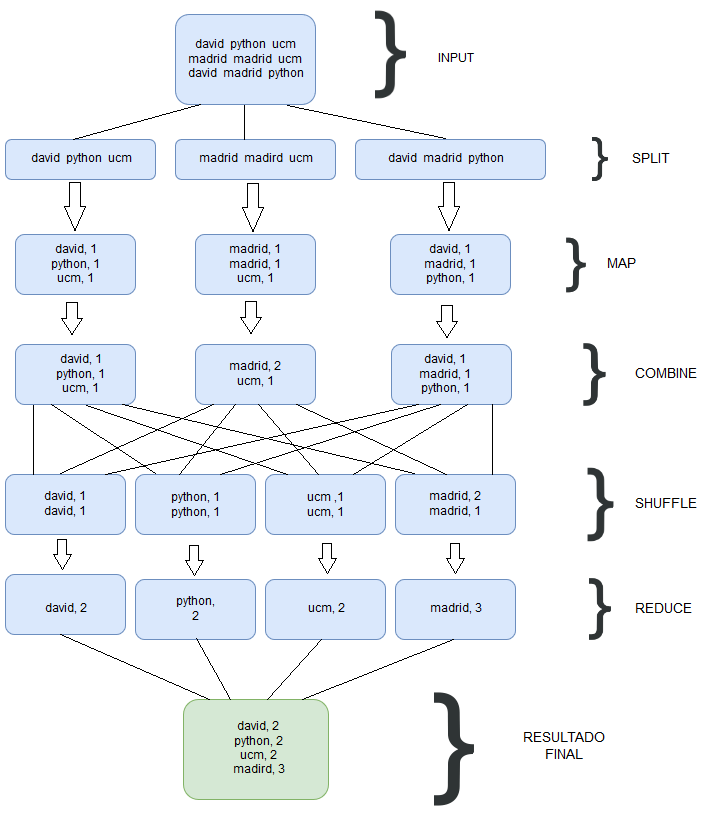
\includegraphics[scale=0.6]{C:/Users/David/Desktop/TFG/TFGLatex/imagenes/mapReduce_wordcount.png}
  \caption[Conteo de palabras en \textit{MapReduce}]{Funcionamiento interno de un \textit{word count} en \textit{MapReduce}}
  \label{mapReduce_wordcount}
\end{figure}

\clearpage

% Apache Spark
\begin{description}
  \item[\textit{Apache Spark}\index{Apache!Spark}:] es un \textit{framework} de procesamiento 
  distribuido para grandes cantidades de datos. Su diseño se basa en funciones del paradigma de programación 
  funcional, realizando los cálculos en memoria, lo que le da mayor rapidez que los motores basados en disco 
  como \textit{MapReduce}.\\
  \textit{Spark} pretende sustituir a \textit{MapReduce} como motor de procesamiento debido a su 
  mayor rendimiento, sobre todo en algoritmos iterativos, lo que acelera mucho el entrenamiento 
  de algoritmos de \textit{machine learning}.
  \textit{Spark} consta de varias librerías como \textit{ML} o \textit{MLlib} para \textit{machine learning} y 
  \textit{GraphX} para el trabajo con grafos.
  La abstracción de procesamiento en \textit{Spark} es el \textbf{RDD} (\textit{Resilient Distributed Dataset}), 
  siendo altamente escalable y tolerante a fallos (mediante puntos de control o \textit{checkpoints}).
  Además, \textit{Spark} soporta \textit{YARN} como gestor de recursos del \textit{cluster}.
  \textit{Apache Spark} es un proyecto de la \textit{Apache Software Foundation} de código abierto, descargable a 
  través de \url{https://spark.apache.org/}
\end{description}


\begin{figure}[!htpb]
  \centering
  
\includegraphics[scale=0.5]{C:/Users/David/Desktop/TFG/TFGLatex/imagenes/apache_spark.png}
  \caption[Logo \textit{Apache Spark}]{Logo de \textit{Apache Spark}}
  \label{spark-devs1}
\end{figure}

% Instalación de MRJOB
La instalación de \textit{Spark} en el \textit{cluster} se detalla en la \autoref{sec:instalacion_spark},
mientras que para la instalación de \textit{mrjob} en la máquina que hemos designado como \textit{gateway},
solo tendremos que lanzar un sencillo comando.\\

\begin{lstlisting}[language=bash, numbers=none]
$ sudo pip install mrjob
\end{lstlisting}

\textit{Pip}\footnote{\textit{Python Package Index}, \url{https://pypi.python.org/pypi/pip}.}, 
el gestor de paquetes de \textit{Python}, se encargará de descargar todas las dependencias
 necesarias para su correcta instalación.

\begin{figure}[!htpb]
  \centering
  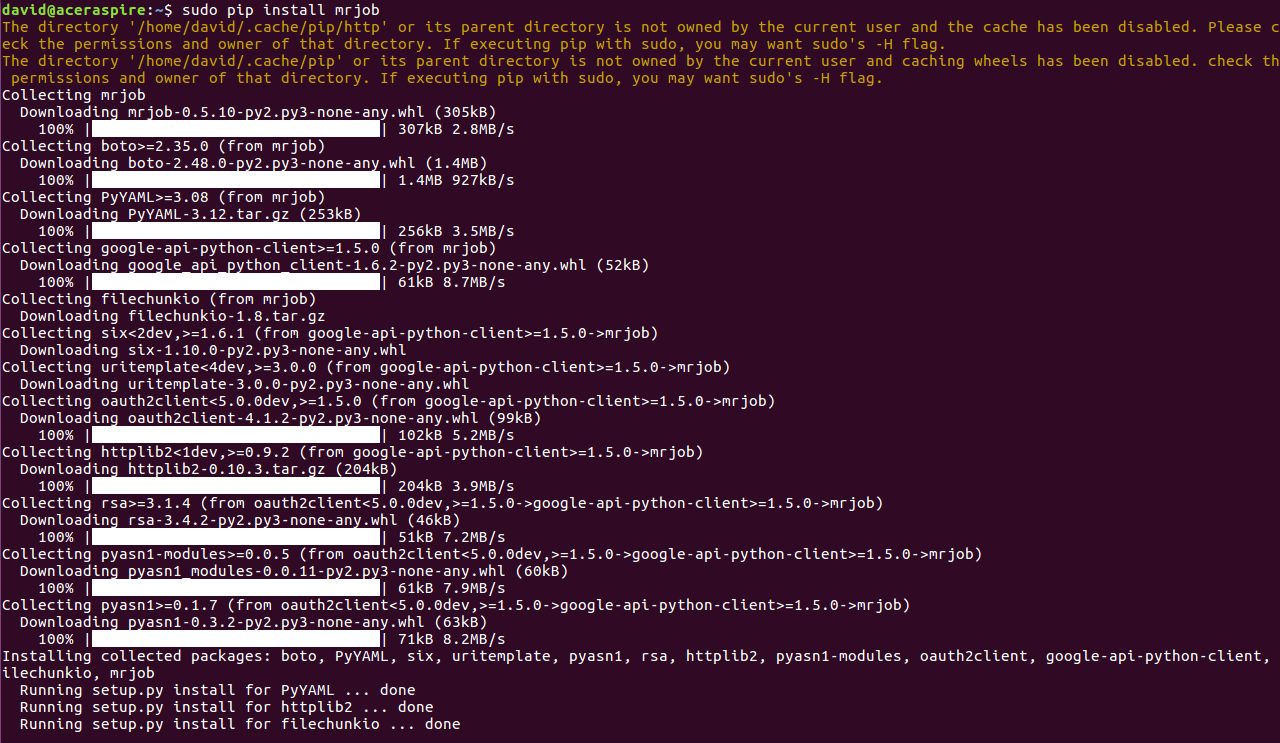
\includegraphics[width=\textwidth]{C:/Users/David/Desktop/TFG/TFGLatex/imagenes/sudo_pip_install_mrjob.png}
  \caption[Instalación de \textit{mrjob}]{Instalación de \textit{mrjob}}
  \label{sudo_pip_install_mrjob}
\end{figure}

\clearpage